\begin{wrapfigure}{r}{0.45\textwidth}
\centering
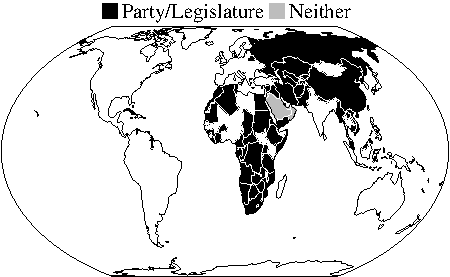
\includegraphics[width=\linewidth]{./sections/01intro/worldmapTermpaperIntro.pdf}
\caption{Parties and legislatures in authoritarian regimes, 2004}
\label{fig:worldmapIntro}
\end{wrapfigure}
Research holds that co-optation and political repression
are two mainstays of authoritarian rule
\citep[21f.]{Gerschewski.2013}. The former is usually 
defined as ``the intentional extension of benefits to 
potential challengers to the regime in exchange for their 
loyalty'' \citep[333]{Frantz.2014}. Legislatures and 
political parties are said to simplify such exchanges. After
the end of the Cold War those nominally democratic
institutions sprung up in almost every authoritarian
regime, and by 2004 only Saudi Arabia, Oman, the
United Arab Emirates, and Qatar sustained neither political 
parties nor a parliament. Yet, authoritarian regimes did not 
forget about political repression. Restrictions on 
political liberties and violations of physical integrity 
rights are pervasive in authoritarian politics. However,
little is know about how co-optation affects political 
repression.

This is the point of departure for Erica Frantz' and Andrea 
Kendall-Taylor's \citeyearpar{Frantz.2014} `A dictator’s 
toolkit: Understanding how co-optation affects repression in 
autocracies'. Based on extensive quantitative analyses they 
argue that increasing levels of co-optation lead dictators 
to reduce restrictions on empowerment rights, but 
simultaneously they increase physical integrity violations
\citep[332]{Frantz.2014}. The authors explain their 
key finding with the trade-offs involved in political 
repression. Restrictions on empowerment rights aim at the 
general public and characterize a diffuse approach to
social control. Physical integrity violations in contrast 
target specific individuals and are attractive when the 
opposition is known. Nominally democratic institutions offer
fora where regime opponents can raise demands, and
thus they generate knowledge on the strength of the 
political opposition. Under the bottom line, 
institutionalized co-optation generates knowledge on threats
to the regime and leads dictators to prefer physical 
integrity violations over empowerment rights restrictions 
\citep[337]{Frantz.2014}.

This paper replicates the work of Frantz and Kendall-Taylor.
It presents evidence on the violation of a key statistical 
assumption, it shows the weak predictive power of the 
original analysis, and it criticizes the use of 
over-parameterized statistical models. My revision
of the original analysis probes the interaction between 
physical integrity violations and co-optation more directly.
As government respect for the integrity of person decreases 
the credibility of political parties and parliaments 
diminishes. Hence, their liberating impact on empowerment 
rights should decrease as physical integrity violations 
intensify. Section two describes design and data of the 
original publication, and section three presents the 
replication results. Section four discusses my modified 
model, and section five concludes.